% chapters/data.tex
\chapter{Data}
\label{ch:data}

% ---------- Chapter 3: Data ----------

\begin{figure}
\centering
    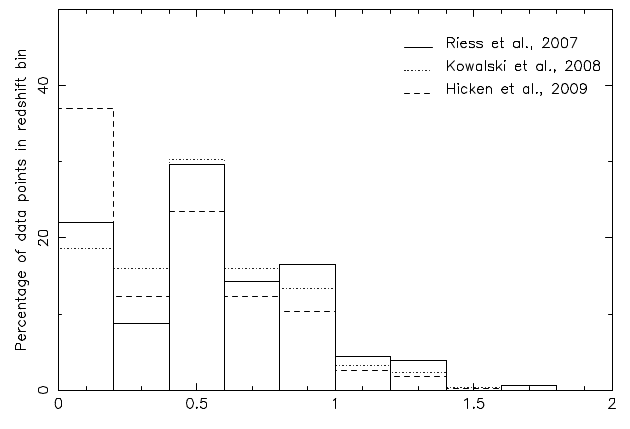
\includegraphics[]{figures/chapter3/fig3.1.png}
\caption{Percentage of SNe Ia from Gold (solid), Union (dotted) and Constitution (dashed) samples falling into redshift bins of width $\Delta z = 0.2$. There are 397 SNe Ia in the Constitution set, 307 SNe Ia in the Union compilation and 182 SNe Ia in the Gold data set. Image credit: \cite{Kwan2009} Fig. 2.}
\label{fig:3.1}
\end{figure}

Type Ia SNe are regarded as the most useful method of determining distances on cosmological scales \cite{Hicken2009}, which makes them ideal candidates for analysing distance-redshift relations. Observational data available for the study was limited: the requirements and three sets which fulfilled them are discussed in \cref{sec:3.1}. A series of projected sets were also made: \cref{sec:3.2} the same samples as the existing sets but with less error and two sets modelled on the expected capability of the \snap{}/\textsc{wfirst} mission.

\section{Observational data}
\label{sec:3.1}

Existing large-scale surveys of Ia SNe are widely used to constrain cosmological parameters, both individually (\cite{Barnes2005,Hicken2009,Kowalski2008,Riess2007}) and in conjunction with other data (\cite{LewisBridle2002,Komatsu2010}). 

The astrophysical properties required for an accurate determination of the parameters place statistical constraints on the available data and how it is processed. Leibundgut emphasises that Ia SNe are cosmologically useful precisely because they map the expansion properties of the universe over a significant fraction of its age (\cite{Leibundgut2008}), with the most recent survey \cite{Amanullah2010} providing Ia SNe luminosity distances out to $z \sim{} 1.5$ (corresponding to a look-back time of about 2/3 of the age of the universe). 
Consequently we require a catalogue of both low- and high-redshift SNe, which in practice is an amalgamation of two (or more) different surveys that require uniform calibration \cite{Kowalski2008}. Furthermore, the quality of spectroscopic data has increased rapidly since the first surveys in the mid-90s (see \cite{Leibundgut2008} for a summary) and we wish to prevent the presence of low-quality data reducing the effectiveness of the higher-quality samples. Implicit in this requirement is a divide between \lq\lq{}good\rq\rq{} and \lq\lq{}bad\rq\rq{} data, which should be made with clearly-defined criteria over all sets, rather than relying on the divides provided by the individual groups \cite{Kowalski2008}. 
Lastly, all spectroscopic data should be analysed with the same light-curve fitting model, so that magnitudes (and therefore luminosity distances) are uniformly calibrated. 

This project is concerned with the data after all of these goals is achieved: it is sufficient to state that each of the three SNe sets satisfied these properties at the time of publication. (The interested reader should consult the introduction of Kowalski’s paper \cite{Kowalski2008} for a more detailed account of how such goals are achieved in practice.) 

Three data sets (\cref{fig:3.1}) which fulfilled these requirements (selected by my supervisor) are the 2006 Gold sample of Riess et al. \cite{Riess2007}, the 2008 Union sample from the Supernova Cosmology Project \cite{Kowalski2008} and the 2009 Constitution sample from Hicken et al \cite{Hicken2009}. In early May 2010 due to \cite{Lidman2010b} I became aware of an even larger suitable set (Union 2) \cite{Amanullah2010}, but it was too late to incorporate this set directly. 

The first sample is the result of two observing periods by Riess et al. using the Advanced Camera for Surveys on the Hubble space telescope \cite{Riess2007}. The use of HST for the whole survey solves two problems: there are no atmospheric effects imprinted on the light curves \cite{Riess2007} and it there was no need to calibrate observational errors across different telescopes \cite{Leibundgut2008}. After uniform calibration and removal of local SNe ($z \lesssim{} 0.02$£, too nearby to be in the Hubble flow) the entire sample was separated into a \lq\lq{}Gold\rq\rq{} set containing SNe which had been positively identified as Type Ia using spectroscopic data and a \lq\lq{}Silver\rq\rq{} set of SNe whose type was unconfirmed \cite{Riess2007}. The Gold set comprises 182 Ia SNe of which 23 are at $z \geq{} 1$. 

The Union set of Kowalski et al. aimed to augment the existing sample of low-$z$ SNe (those in the nearby Hubble flow), since this is a region of smooth ($H(z) \sim{}$ constant) expansion, the $H(z)$ value of which was not well constrained at the time \cite{Kowalski2008}). It is mainly a uniform re-analysis of 414 SNe Ia (reduced to 307 after light-curve quality cuts) which already existed in the literature \cite{Kwan2009}: data from the first year of the two large, ground-based surveys of the time (the Supernova Legacy Survey and the ESSENCE survey) and previous surveys from a variety of instruments, including 17 SNe Ia from the Gold sample \cite{Kowalski2008}. 

The Union set is a proper subset of the Constitution set, which also contains SNe from around seven different surveys collectively known as the CfA3 set \cite{Hicken2009}. The addition of 90 Ia SNe from the CfA3 set increased the number of low-$z$ SNe by a factor of $2.6 -- 2.9$: the sample size was now sufficiently large for systematic errors to be the dominant contributor to distance modulus uncertainties \cite{Hicken2009}. According to Kwan all three data sets are consistent with one another, despite the gold set intersecting with, rather than being a subset of the other two \cite{Kwan2009}.

\section{Artificially generated data}
\label{sec:3.2}

This data falls into two categories: modification of existing data and creation of speculative projected sets. 

These represent the two major directions of future SNe cosmology: re-analysis of existing, heterogeneous data using uniform light curves and collection of new, homogeneous data from large surveys. 

The smaller-error samples (Gold 02, Union 02 and Constitution 02) were created by taking the existing data and reducing the distance modulus uncertainty $\Delta{} \mu$ fivefold. This improvement represents a reduction of systematic errors currently encountered in survey data reduction. This reduction may arise from two different areas: improvement of experimental systematics --- Malmquist bias, $k$-correction uncertainties, sample contamination with non-SNe Ia, possible gravitational lensing --- and better understanding of the SNe themselves --- different populations in different environments, evolution with redshift, possible metallicity-luminosity relation \cite{Lidman2010b}. 

Comparison of these smaller-error sets with the real ones will determine how much uncertainties in luminosity distance contribute to uncertainty in the cosmological parameters. The projected sets represent hypothetical data from the planned \textsc{wfirst} mission (previous \snap{}, then \textsc{jdem}), which has been given top priority in the recent US decadal survey \cite{Blandford2010}. The \textsc{wfirst} project consists of a space-based 1.5m telescope for photometric discovery of distant Ia SNe with ground-based spectroscopic confirmation combined with a ground-based survey of near (Hubble flow) SNe \cite{Albrecht2006}. It anticipates surveying 2000 SNe in redshifts $0.1 < z < 1.7$ \cite{Blandford2010}. The method used to generate the false data is described in \cref{sec:4.2} with the rest of the numerical work (\cref{ch:numerical-modelling}).
